\documentclass[a4paper]{article}

\usepackage[polish]{babel}
\usepackage[utf8]{inputenc}
\usepackage{polski}
\usepackage{amsmath}
\usepackage{graphicx}
\usepackage[parfill]{parskip}
\usepackage{float}
\usepackage{multirow}
\usepackage[normalem]{ulem}
\usepackage{lmodern}  % for bold teletype font
\usepackage{amsmath}  % for \hookrightarrow
\usepackage{xcolor}   % for \textcolor
\usepackage{listings}
\lstset{
	basicstyle=\ttfamily,
	columns=fullflexible,
	breaklines=true,
	postbreak=\mbox{\textcolor{red}{$\hookrightarrow$}\space},
}

\title{Bezpieczeństwo usług sieciowych \\ --- laboratorium 4 --- \\ crackme}

\author{Adrian Frydmański}

\date{\today}

\begin{document}
	\maketitle
	
	\section{Zadanie do wykonania}
	Zadaniem była zmiana kodu binarki na poziomie bitów, by program wykonał się tak, jak chce tego autor -- wykonał funkcję \texttt{winner}.
	
	\section{Kroki prowadzące do rozwiązania}
	Deasemblacja wymagała wpisania \texttt{objdump -D crackme}. Pierwszym -- i całkiem trafnym -- pomysłem była podmiana adresu wywoływanej funkcji. Oto adresy, na które można było zwrócić uwagę:
	\begin{itemize}
		\item sekcja \texttt{<cheater>} -- 80484e2
		\item sekcja \texttt{<winner>} -- 8048566
		\item sekcja \texttt{<looser>} -- 8048552 
		\item sekcja \texttt{<init>} -- 804857a
		\item wywołanie \texttt{<init>} w \texttt{<main>} -- 80485be
		\item wywołanie \texttt{<cheater>} w \texttt{<main>} -- 80485cc
	\end{itemize}

	\subsection{Sposób 1}

	Proponowaną zmianą jest podmiana adresu \texttt{<init>} na \texttt{<winner>} w wywołaniu \texttt{<init>} w \texttt{<main>}:
	
	\begin{lstlisting}[caption={Fragment objdumpa}, captionpos=b]
08048552 <looser>:
 8048552:	55                   	push   %ebp
 8048553:	89 e5                	mov    %esp,%ebp
 8048555:	83 ec 18             	sub    $0x18,%esp
 8048558:	c7 04 24 63 87 04 08 	movl   $0x8048763,(%esp)
 804855f:	e8 74 fe ff ff       	call   80483d8 <puts@plt>
 8048564:	c9                   	leave  
 8048565:	c3                   	ret    

08048566 <winner>:
 8048566:	55                   	push   %ebp
 8048567:	89 e5                	mov    %esp,%ebp
 8048569:	83 ec 18             	sub    $0x18,%esp
 804856c:	c7 04 24 78 87 04 08 	movl   $0x8048778,(%esp)
 8048573:	e8 60 fe ff ff       	call   80483d8 <puts@plt>
 8048578:	c9                   	leave  
 8048579:	c3                   	ret    

080485b5 <main>:
 80485b5:	55                   	push   %ebp
 80485b6:	89 e5                	mov    %esp,%ebp
 80485b8:	83 e4 f0             	and    $0xfffffff0,%esp
 80485bb:	83 ec 30             	sub    $0x30,%esp
 80485be:	e8 b7 ff ff ff       	call   804857a <init>
 80485c3:	e8 dc fe ff ff       	call   80484a4 <time_guard>
 80485c8:	85 c0                	test   %eax,%eax
 80485ca:	74 0a                	je     80485d6 <main+0x21>
 80485cc:	e8 11 ff ff ff       	call   80484e2 <cheater>
	\end{lstlisting}
	
	W celu edycji posłużyłem się programem do edycji plików binarnych Jeex. Wyszukałem adres sekcji (funkcji) w pliku na podstawie danych z objdumpa. Wystepował tylko raz, więc miałem pewność, że to ten.
	
	\begin{figure}[H]
		\centering
		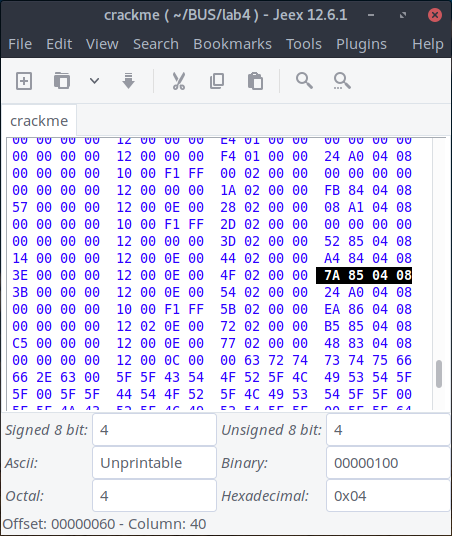
\includegraphics[width=.4\textwidth]{img/init_addr}
		\caption{Znaleziony adres funkcji init}
	\end{figure}

	Na co należało zwrócić uwagę, to fakt, iż przy wyszukiwaniu adresu trzeba zmienić kolejność bajtów, gdyż w pliku binarnym są podawane od najmłodszego.
	
	\begin{figure}[H]
		\centering
		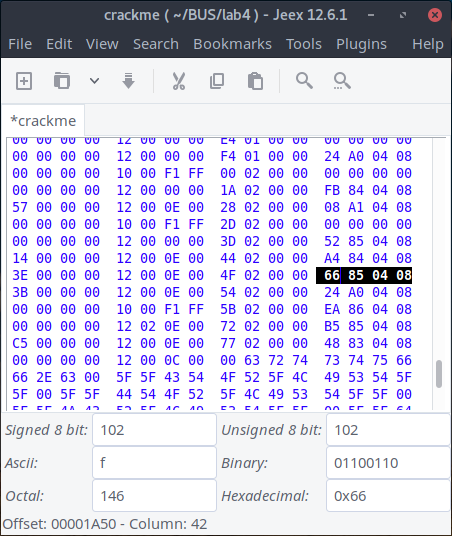
\includegraphics[width=.4\textwidth]{img/winner_addr}
		\caption{Adres funkcji init zmieniony na adres funkcji winner}
	\end{figure}

	Ostatecznie zmianie uległ najmłodszy bajt adresu -- z \texttt{0x7a} (\texttt{01100011b}) na \texttt{0x66} (\texttt{01111000b}) -- co dało 4 zmienione bity.
	
	Funkcje \texttt{<winner>} i \texttt{<looser>} są prawie takie same i można w nich zamienić adres tekstku drukowanego na ekran przez wywołanie \texttt{<puts@plt>}.
	
	\begin{figure}[H]
		\centering
		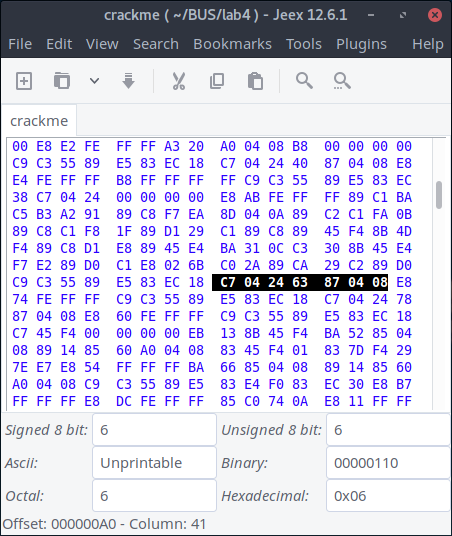
\includegraphics[width=.4\textwidth]{img/looser_str_addr}
		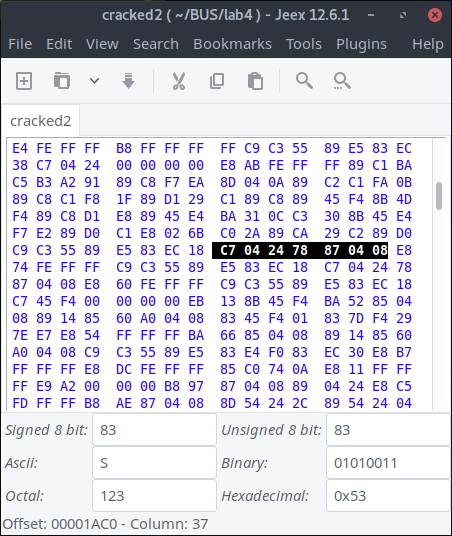
\includegraphics[width=.4\textwidth]{img/winner_str_addr}
		\caption{Adresy stringów drukowanych na ekran}
	\end{figure}

	W efekcie tego działania po wpisaniu dowolnego znaku (lub znaków) wywoływana jest funkcja winner.
	
	\begin{figure}[H]
		\centering
		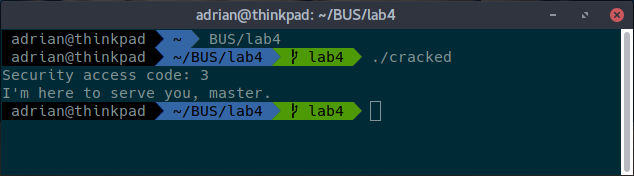
\includegraphics[width=.5\textwidth]{img/result}
		\caption{Wynik działania ze zmeinionym adresem funkcji}
	\end{figure}

	Taki efekt w momencie pisania sprawozdania był możliwy po zmianie czasu systemu przez porównywanie czasu w programie z timestampem z dnia zajęć.
	
	\subsection{Sposób 2}
		
	Jest też inna możliwość. Można zamienić pierwsze wywołanie \texttt{<cheater>} w \texttt{<main>} na wywołenie \texttt{<winner>}. W callu jest przesunięcie względem aktualnego adresu. Instrukcję
	\texttt{80485cc:	e8 11 ff ff ff       	call   80484e2 <cheater>}
	należy zamienić na \texttt{e8 95 ff ff ff} -- przy zmianie \texttt{11} (\texttt{00010001}) na \texttt{95} (\texttt{10010101}) uzyskujemy zmianę tylko 2 bitów. Wynika to z różnicy w adresach: $0x080484e2 - 0x08048566 = 0x84$.
	Tyle właśnie należało dodać do przesunięcia -- początkowo oznaczonego jako 0x11 w instrukcji -- aby przenieść się o 0x84 dalej, do funkcji \texttt{<winner>}.
	Niestety takie wykonanie programu kończy się tak, jak w przypadku otrzymania komunikatu o błędzie -- z inną od zera zwróconą wartością -- i było możliwe dopiero po zakończeniu zajęć laboratoryjnych albo po zmianie daty w systemie.
	
	\begin{figure}[H]
		\centering
		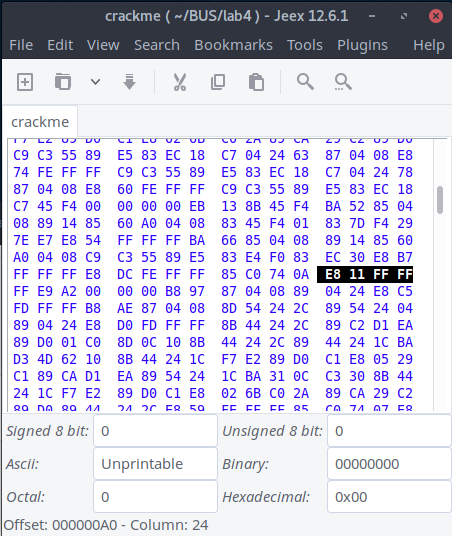
\includegraphics[width=.4\textwidth]{img/magia1}
		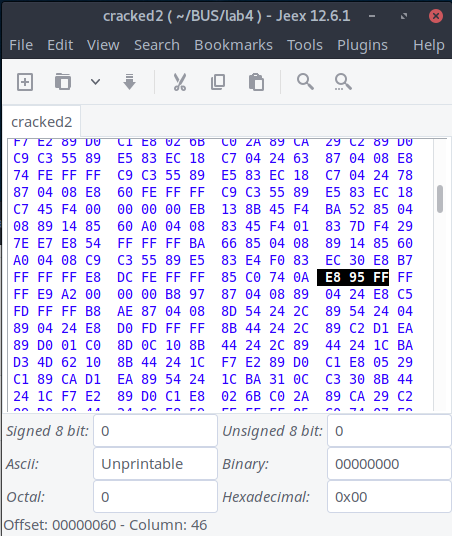
\includegraphics[width=.4\textwidth]{img/magia2}
		\caption{Zmiana calla}
	\end{figure}

	\begin{figure}[H]
		\centering
		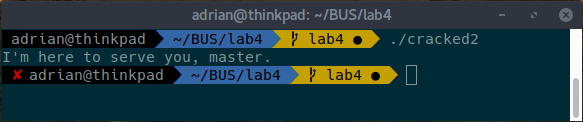
\includegraphics[width=.5\textwidth]{img/magia_result}
		\caption{Wynik działania ze zmienionym callem}
	\end{figure}

	\section{Podsumowanie}
	Zadanie pokazało kolejne ciekawe aspekty wynikające ze znajomości assemblera i umiejętności operowania na plikach binarnych.
	
	Plik \texttt{cracked} zawiera binarkę zmienioną pierwszym sposobem, zaś \texttt{cracked2} -- drugim.
	
\end{document}